% ============================================================
\chapter{Analyse de Sensibilit\'e}
\label{ch:sensibilite}
% ============================================================

Un mod\`ele d'optimisation n'est jamais parfait~: les co\^uts, les capacit\'es, les demandes sont estim\'es, et ces estimations comportent des marges d'erreur. La question naturelle est~: jusqu'\`a quel point la solution optimale reste-t-elle valide si les param\`etres changent l\'eg\`erement~? C'est la question de l'\emph{analyse de sensibilit\'e}, un outil indispensable pour le d\'ecideur. Gr\^ace \`a la structure du simplexe et \`a la dualit\'e, on peut r\'epondre \`a cette question sans r\'esoudre un nouveau probl\`eme~: il suffit d'examiner les intervalles de variation des param\`etres pour lesquels la base optimale reste inchang\'ee.

\section{Introduction}

En pratique, les param\`etres d'un PL (co\^uts $c_j$, ressources $b_i$,
coefficients $a_{ij}$) ne sont jamais connus avec une pr\'ecision absolue.
L'\textbf{analyse de sensibilit\'e} \'etudie comment la solution optimale
et la valeur optimale varient lorsque ces param\`etres changent.

\begin{definition}[Analyse de sensibilit\'e]
L'\textbf{analyse de sensibilit\'e} (ou \textbf{analyse post-optimale})
d\'etermine les intervalles de variation des param\`etres pour lesquels
la \textbf{base optimale} reste inchang\'ee.
\end{definition}

\section{Variation des membres droits $b_i$}

\subsection{Effet sur la solution}

Soit $\mathbf{b}' = \mathbf{b} + \Delta\mathbf{b}$.  La solution de base
reste~:
\[
  \mathbf{x}_B' = B^{-1}\mathbf{b}' = B^{-1}\mathbf{b} + B^{-1}\Delta\mathbf{b}
  = \bar{\mathbf{b}} + B^{-1}\Delta\mathbf{b}
\]

La base reste r\'ealisable tant que $\mathbf{x}_B' \ge \mathbf{0}$, soit~:
\[
  \bar{\mathbf{b}} + B^{-1}\Delta\mathbf{b} \ge \mathbf{0}
\]

\subsection{Variation d'un seul $b_i$}

Si seul $b_i$ varie d'un montant $\delta$~:
\[
  \bar{b}_k + (B^{-1})_{ki} \cdot \delta \ge 0, \quad k = 1, \ldots, m
\]

\begin{formules}[title=\textbf{Intervalle de validit\'e de $b_i$}]
La base reste optimale pour~:
\[
  b_i \in \left[
    b_i - \min_{k:\, (B^{-1})_{ki}>0} \frac{\bar{b}_k}{(B^{-1})_{ki}},\;
    b_i + \min_{k:\, (B^{-1})_{ki}<0} \frac{-\bar{b}_k}{(B^{-1})_{ki}}
  \right]
\]
\end{formules}

\begin{theoreme}[Variation de $z^*$]
Lorsque $b_i$ varie de $\delta$ dans l'intervalle de validit\'e~:
\[
  z^*(\delta) = z^* + y_i^* \cdot \delta
\]
o\`u $y_i^*$ est le prix fictif (variable duale) de la contrainte $i$.
\end{theoreme}

\begin{exemple}[Variation de $b_1$]
Reprenons le PL du chapitre~3~:
\[
\max\ z = 5x_1 + 4x_2 \quad \text{s.c.} \quad
6x_1 + 4x_2 \le 24,\; x_1 + 2x_2 \le 6
\]

Le tableau final donne $B^{-1} = \begin{pmatrix} 1/4 & -1/2 \\
-1/8 & 3/4 \end{pmatrix}$, $\bar{\mathbf{b}} = (3, 3/2)^\top$,
$y_1^* = 3/4$, $y_2^* = 1/2$.

Pour la variation de $b_1 = 24$~:
\begin{itemize}
  \item $(B^{-1})_{11} = 1/4 > 0$~: $\delta \ge -\bar{b}_1/(1/4) = -12$
  \item $(B^{-1})_{21} = -1/8 < 0$~: $\delta \le -\bar{b}_2/(-1/8) = 12$
\end{itemize}
Donc $b_1 \in [24-12, 24+12] = [12, 36]$.

Si $b_1 = 30$~: $z^*(30) = 21 + (3/4)(30-24) = 21 + 4.5 = 25.5$.
\end{exemple}

\section{Variation des coefficients de l'objectif $c_j$}

\subsection{Variable de base}

Si $x_j$ est une variable de base, la variation de $c_j$ affecte les
co\^uts r\'eduits des variables hors-base.  La base reste optimale tant que
tous les co\^uts r\'eduits restent $\ge 0$ (minimisation) ou $\le 0$
(maximisation dans le tableau).

\begin{formules}[title=\textbf{Intervalle de validit\'e de $c_j$ (variable de base)}]
Les co\^uts r\'eduits des variables hors-base $k$ deviennent~:
\[
  \bar{c}_k' = \bar{c}_k - \delta \cdot \bar{a}_{rk}
\]
o\`u $r$ est la ligne de $x_j$ dans la base et $\delta = c_j' - c_j$.
La base reste optimale pour $\bar{c}_k' \ge 0$ pour tout $k$ hors-base.
\end{formules}

\subsection{Variable hors-base}

Si $x_j$ est hors-base avec $\bar{c}_j > 0$ (maximisation), la base reste
optimale tant que $\bar{c}_j + \delta \ge 0$, soit
$c_j \ge c_j - \bar{c}_j$.

\begin{exemple}[Variation de $c_1$]
Dans notre exemple, $x_1$ est de base.  Les co\^uts r\'eduits des variables
hors-base ($s_1, s_2$) dans le tableau final sont~:
$\bar{c}_{s_1} = 3/4$, $\bar{c}_{s_2} = 1/2$.

La ligne de $x_1$ donne $\bar{a}_{1,s_1} = 1/4$, $\bar{a}_{1,s_2} = -1/2$.

\begin{itemize}
  \item $\bar{c}_{s_1}' = 3/4 - \delta(1/4) \ge 0 \Rightarrow \delta \le 3$
  \item $\bar{c}_{s_2}' = 1/2 - \delta(-1/2) = 1/2 + \delta/2 \ge 0
        \Rightarrow \delta \ge -1$
\end{itemize}
Donc $c_1 \in [5-1, 5+3] = [4, 8]$.
\end{exemple}

\section{Ajout d'une nouvelle variable}

Si l'on ajoute une variable $x_{n+1}$ avec co\^ut $c_{n+1}$ et colonne
technologique $\mathbf{a}_{n+1}$, on calcule~:
\[
  \bar{c}_{n+1} = c_{n+1} - \mathbf{c}_B^\top B^{-1} \mathbf{a}_{n+1}
\]

\begin{itemize}
  \item Si $\bar{c}_{n+1} \ge 0$ (minimisation)~: la solution reste
        optimale sans utiliser $x_{n+1}$.
  \item Si $\bar{c}_{n+1} < 0$~: il est avantageux de faire entrer
        $x_{n+1}$ en base.
\end{itemize}

\section{Ajout d'une nouvelle contrainte}

Si l'on ajoute une contrainte $\mathbf{a}_{m+1}^\top \mathbf{x} \le b_{m+1}$~:
\begin{enumerate}
  \item V\'erifier si la solution optimale actuelle $\mathbf{x}^*$ satisfait
        la nouvelle contrainte~: $\mathbf{a}_{m+1}^\top \mathbf{x}^* \le b_{m+1}$.
  \item Si oui~: la solution reste optimale.
  \item Si non~: appliquer le \textbf{simplexe dual} en ajoutant la contrainte
        (avec une variable d'\'ecart) au tableau final.
\end{enumerate}

\section{Analyse param\'etrique}

\begin{definition}[Analyse param\'etrique]
L'\textbf{analyse param\'etrique} \'etudie la variation continue de $z^*$
en fonction d'un param\`etre $\theta$~:
\[
  \mathbf{b}(\theta) = \mathbf{b} + \theta \mathbf{d}
  \qquad \text{ou} \qquad
  \mathbf{c}(\theta) = \mathbf{c} + \theta \mathbf{e}
\]
o\`u $\mathbf{d}$ ou $\mathbf{e}$ sont des directions fix\'ees.
\end{definition}

\begin{theoreme}[Forme de $z^*(\theta)$]
La valeur optimale $z^*(\theta)$ est une fonction \textbf{lin\'eaire par
morceaux} et \textbf{concave} (si on fait varier $\mathbf{b}$ en
maximisation) de $\theta$.  Chaque segment correspond \`a une base optimale
diff\'erente.
\end{theoreme}

\begin{center}
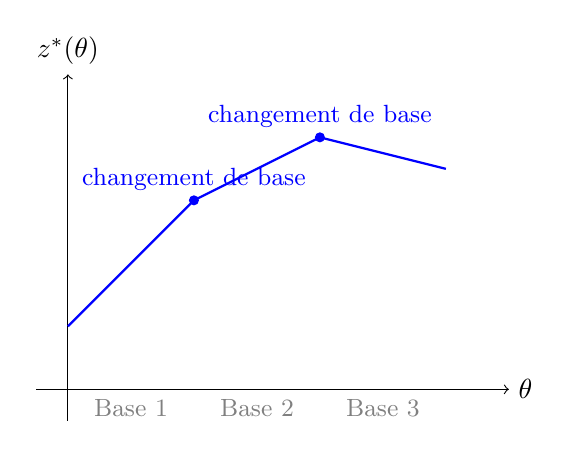
\begin{tikzpicture}[scale=0.8]
  \draw[->] (-0.5,0) -- (7,0) node[right] {$\theta$};
  \draw[->] (0,-0.5) -- (0,5) node[above] {$z^*(\theta)$};
  \draw[thick, blue] (0,1) -- (2,3) -- (4,4) -- (6,3.5);
  \filldraw[blue] (2,3) circle (2pt) node[above] {\small changement de base};
  \filldraw[blue] (4,4) circle (2pt) node[above] {\small changement de base};
  \node[gray, below] at (1,0) {\small Base 1};
  \node[gray, below] at (3,0) {\small Base 2};
  \node[gray, below] at (5,0) {\small Base 3};
\end{tikzpicture}
\end{center}

\section{Impl\'ementation Python}

\begin{codeblock}[title=\textbf{Analyse de sensibilit\'e avec SciPy}]
\begin{minted}{python}
from scipy.optimize import linprog
import numpy as np

c = [-5, -4]  # max 5x1 + 4x2
A_ub = [[6, 4], [1, 2]]
b_ub = [24, 6]
bounds = [(0, None), (0, None)]

# Solution de base
res = linprog(c, A_ub=A_ub, b_ub=b_ub, bounds=bounds,
              method='highs')
print(f"z* = {-res.fun:.2f}, x* = {res.x}")

# Sensibilité de b1
print("\nVariation de b1 :")
for delta in [-12, -6, 0, 6, 12]:
    b_new = [24 + delta, 6]
    r = linprog(c, A_ub=A_ub, b_ub=b_new, bounds=bounds,
                method='highs')
    print(f"  b1={24+delta:3d} -> z*={-r.fun:.2f}, "
          f"x*=[{r.x[0]:.2f}, {r.x[1]:.2f}]")

# Sensibilité de c1
print("\nVariation de c1 :")
for c1 in [3, 4, 5, 6, 8]:
    c_new = [-c1, -4]
    r = linprog(c_new, A_ub=A_ub, b_ub=b_ub, bounds=bounds,
                method='highs')
    print(f"  c1={c1} -> z*={-r.fun:.2f}, "
          f"x*=[{r.x[0]:.2f}, {r.x[1]:.2f}]")
\end{minted}
\end{codeblock}

\begin{codeoutput}
z* = 21.00, x* = [3.  1.5]

Variation de b1 :
  b1= 12 -> z*= 12.00, x*=[0.00, 3.00]
  b1= 18 -> z*= 16.50, x*=[1.50, 2.25]
  b1= 24 -> z*= 21.00, x*=[3.00, 1.50]
  b1= 30 -> z*= 25.50, x*=[4.50, 0.75]
  b1= 36 -> z*= 30.00, x*=[6.00, 0.00]

Variation de c1 :
  c1=3 -> z*= 15.00, x*=[3.00, 1.50]
  c1=4 -> z*= 18.00, x*=[3.00, 1.50]
  c1=5 -> z*= 21.00, x*=[3.00, 1.50]
  c1=6 -> z*= 24.00, x*=[3.00, 1.50]
  c1=8 -> z*= 30.00, x*=[3.00, 1.50]
\end{codeoutput}

\section{Rapport de sensibilit\'e}

Les solveurs commerciaux fournissent un \textbf{rapport de sensibilit\'e}
contenant pour chaque contrainte et chaque variable~:

\begin{center}
\renewcommand{\arraystretch}{1.2}
\begin{tabular}{lp{8cm}}
  \toprule
  \textbf{Information} & \textbf{Description} \\
  \midrule
  Valeur optimale & Valeur de la variable/contrainte \`a l'optimum \\
  Prix fictif (shadow price) & Variation marginale de $z^*$ par unit\'e de $b_i$ \\
  Co\^ut r\'eduit & Variation marginale n\'ecessaire de $c_j$ pour que
                    $x_j$ entre en base \\
  Augmentation admissible & Borne sup\'erieure de variation \\
  Diminution admissible & Borne inf\'erieure de variation \\
  \bottomrule
\end{tabular}
\end{center}

\section{Exercices}

\begin{exercice}[$\star$ -- Intervalles de validit\'e]
Pour le PL~:
\[
\max\ z = 3x_1 + 2x_2 \quad \text{s.c.} \quad
x_1 + x_2 \le 10,\; 2x_1 + x_2 \le 14,\; x_1, x_2 \ge 0
\]
D\'eterminer les intervalles de validit\'e de $b_1$ et $b_2$.
\end{exercice}

\begin{exercice}[$\star\star$ -- Variation d'objectif]
Dans le m\^eme PL, d\'eterminer l'intervalle de $c_1$ pour lequel la base
optimale ne change pas.
\end{exercice}

\begin{exercice}[$\star\star$ -- Nouvelle variable]
Doit-on introduire un nouveau produit $P_3$ avec profit $c_3 = 6$ et
consommation $(a_{13}, a_{23}) = (3, 1)$~?
\end{exercice}

\begin{exercice}[$\star\star$ -- Nouvelle contrainte]
On ajoute la contrainte $x_1 + x_2 \le 5$.  La solution optimale
est-elle toujours r\'ealisable~?  Si non, trouver la nouvelle solution
optimale.
\end{exercice}

\begin{exercice}[$\star\star\star$ -- Analyse param\'etrique compl\`ete]
\'Etudier $z^*(\theta)$ pour $\mathbf{b}(\theta) = (10 + \theta, 14 - 2\theta)$
lorsque $\theta$ varie de $-5$ \`a $+5$.  Tracer la courbe et identifier les
changements de base.
\end{exercice}

\begin{exercice}[$\star\star\star$ -- Impl\'ementation]
\'Ecrire un script Python qui~:
\begin{enumerate}
  \item R\'esout un PL avec PuLP.
  \item Calcule automatiquement les intervalles de validit\'e de chaque $b_i$
        par perturbation num\'erique.
  \item Trace le graphe de $z^*(\theta)$ pour une variation param\'etrique
        de $b_1$.
\end{enumerate}
\end{exercice}
